%%%%%%%%%%%%%%%%%%%%%%%%%
% Dokumentinformationen %
%%%%%%%%%%%%%%%%%%%%%%%%%
\newcommand{\titleinfo}{Regelungstechnik 1 - Formelsammlung}
\newcommand{\authorinfo}{Braun \& Co, J\"urg \& DIE Schweisser, C.Gwerder, S.Koerner}
\newcommand{\versioninfo}{$Version: 1.1$}

%%%%%%%%%%%%%%%%%%%%%%%%%%%%%%%%%%%%%%%%%%%%%
% Standard projektübergreifender Header für
% - Makros 
% - Farben
% - Mathematische Operatoren
%
% DORT NUR ERGÄNZEN, NICHTS LÖSCHEN
%%%%%%%%%%%%%%%%%%%%%%%%%%%%%%%%%%%%%%%%%%%%%
% Genereller Header
\documentclass[10pt,twoside,a4paper,fleqn]{article}
\usepackage[utf8]{inputenc}
\usepackage[left=1cm,right=1cm,top=1cm,bottom=1cm,includeheadfoot]{geometry}
\usepackage[ngerman]{babel,varioref}

% Pakete
\usepackage{amssymb,amsmath,fancybox,graphicx,color,lastpage,wrapfig,fancyhdr,hyperref,verbatim,floatflt}


%%%%%%%%%%%%%%%%%%%%
% Generelle Makros %
%%%%%%%%%%%%%%%%%%%%
\newcommand{\formelbuch}[1]{$_{\textcolor{red}{\mbox{\small{S#1}}}}$}
\newcommand{\verweis}[2]{\small{(siehe auch \ref{#1}, #2 (S. \pageref{#1}))}}
\newcommand{\subsubadd}[1]{\textcolor{black}{\mbox{#1}}}


\newcommand{\skriptsection}[2]{\section{#1 {\tiny Skript S. #2}}}
\newcommand{\skriptsubsection}[2]{\subsection{#1 {\tiny Skript S. #2}}}
\newcommand{\skriptsubsubsection}[2]{\subsubsection{#1 {\tiny Skript S. #2}}}

%%%%%%%%%%
% Farben %
%%%%%%%%%%
\definecolor{black}{rgb}{0,0,0}
\definecolor{red}{rgb}{1,0,0}
\definecolor{white}{rgb}{1,1,1}
\definecolor{grey}{rgb}{0.8,0.8,0.8}

%%%%%%%%%%%%%%%%%%%%%%%%%%%%
% Mathematische Operatoren %
%%%%%%%%%%%%%%%%%%%%%%%%%%%%
\DeclareMathOperator{\sinc}{sinc}



% Fouriertransformationen
\unitlength1cm
\newcommand{\FT}
{
\begin{picture}(1,0.5)
\put(0.2,0.1){\circle{0.14}}\put(0.27,0.1){\line(1,0){0.5}}\put(0.77,0.1){\circle*{0.14}}
\end{picture}
}


\newcommand{\IFT}
{
\begin{picture}(1,0.5)
\put(0.2,0.1){\circle*{0.14}}\put(0.27,0.1){\line(1,0){0.45}}\put(0.77,0.1){\circle{0.14}}
\end{picture}
}



%%%%%%%%%%%%%%%%%%%%%%%%%%%%
% Allgemeine Einstellungen %
%%%%%%%%%%%%%%%%%%%%%%%%%%%%
%pdf info
\hypersetup{pdfauthor={\authorinfo},pdftitle={\titleinfo},colorlinks=false}
\author{\authorinfo}
\title{\titleinfo}

%Kopf- und Fusszeile
\pagestyle{fancy}
\fancyhf{}
%Linien oben und unten
\renewcommand{\headrulewidth}{0.5pt} 
\renewcommand{\footrulewidth}{0.5pt}

\fancyhead[L]{\titleinfo{ }\tiny{(\versioninfo)}}
%Kopfzeile rechts bzw. aussen
\fancyhead[R]{Seite \thepage { }von \pageref{LastPage}}
%Fusszeile links bzw. innen
\fancyfoot[L]{\footnotesize{\authorinfo}}
%Fusszeile rechts bzw. ausen
\fancyfoot[R]{\footnotesize{\today}}

% Einrücken verhindern versuchen
\setlength{\parindent}{0pt}


%%%%%%%%%%%%%%%%%%%%%%%%%%%%%%%%%%%%%%%%%%%%%%%%%%%%%%%%%%%%%%%%%%%%%%%%%%%%%%%%%%%%%%%%%%%%%%%%
% Neue Befehle und Definitionen                
%%%%%%%%%%%%%%%%%%%%%%%%%%%%%%%%%%%%%%%%%%%%%%%%%%%%%%%%%%%%%%%%%%%%%%%%%%%%%%%%%%%%%%%%%%%%%%%
\usepackage{enumitem}

\setlist[1]{labelindent=\parindent} % < Usually a good idea
\setlist{style=multiline,topsep=0pt,rightmargin=2cm}
\setlist[enumerate]{leftmargin=0.5cm}



\begin{document}

\section{Technischer Regelkreis}
\subsection{Definitionen}

\begin{description}[leftmargin=2.5cm]
 \item[System] Eine Anordnung von Gebilden, die miteinander in Beziehung stehen
        	   und die sich gegenüber der Umgebung abgrenzen lasen.
 \item[Prozess] Die Gesammtheit der zusammenwirkenden Vorgänge in einem System,
        		durch die Materie, Energie, Informationen umgeformt, transportiert und
        		gespeichert wird.
 \item[SISO] Single Input - Single Output
 \item[MIMO] Multi Input - Multi Output
 \item[Steuerung] ohne Rückkopplung \newline
 				  - kann bei \textbf{stabiler} Strecke \textbf{nicht instabil} werden
 \item[Regelung] mit Rückkopplung (wirkt als Gegenkopplung) \newline
 				 - immer ein Vergleichsglied zwischen Führungsgrösse (Sollwert) und
 				 Regelgrösse (Istwert) \newline
 				 - kann auf veränderte Störgrössen reagieren \newline
 				 - kann bei \textbf{stabiler} Strecke \textbf{instabil} werden.
\end{description}

	\begin{tabular}{|p{2.7cm}|p{5.4cm}|l|}
    	\hline
    	{\bf Begriff deutsch}		&{\bf Begriff englisch}	&{\bf Ergänzende
    	Erklärung}\\
		\hline
		Regelung /
		Regelkreis			& closed loop control / control loop & \\
		\hline
		Regelstrecke
    	Reglekreis			&plant controlled system	&Der aufgabengemäss zu beeinflussende
    	Teil des Systems\\
    	\hline
    	Regler				&controller			&Bestehent aus Vergleichsglied und Regelglied\\
    	\hline
    	Regeleinrichtung	&controlling means&\\
    	\hline
    	Reglesignalkreis	&control circuit&\\
    	\hline
    	Vergleichsglied		&comparing element	&Bildet den Fehler (Differenz)
    											e=r-y\\
    	\hline
    	Regelglied			&controller;
    						controlling element	&Berechnet aus dem Fehler die Stellgrösse u\\
    	\hline
    	Stelleinrichtung
    	Verstärker			&actuator;
					    	power amplifier;
    						servo amplifier		&Funktionseinheit, die den Energie- oder Massenstrom
    											lenkt\\
    	\hline
    	Messeinrichtung
    	Messumformer		&measuring unit;
    						transmitter&\\
    	\hline
    	Regelgrösse y		&controlled variable;
    						desiered value& auch c oder x (DIN)\\
    	\hline
    	Führungsgrösse r	&reference variable;
    						set value& w (DIN)\\
    	\hline
    	Störgrösse z Last	&disturbance variable;
    						load&\\
    	\hline
    	Stellgrösse u		&manipulatetd (correcting)
    						variable& y (DIN)\\
    	\hline
    	Regeldifferenz e
    	Fehler				&deviation;
    						error variable		&$e=r-y \quad \quad x_d=w-x$ (DIN) \\
    	\hline
    	Rückkopplung		&feedback			&Rückführung\\
    	\hline

	\end{tabular}\\
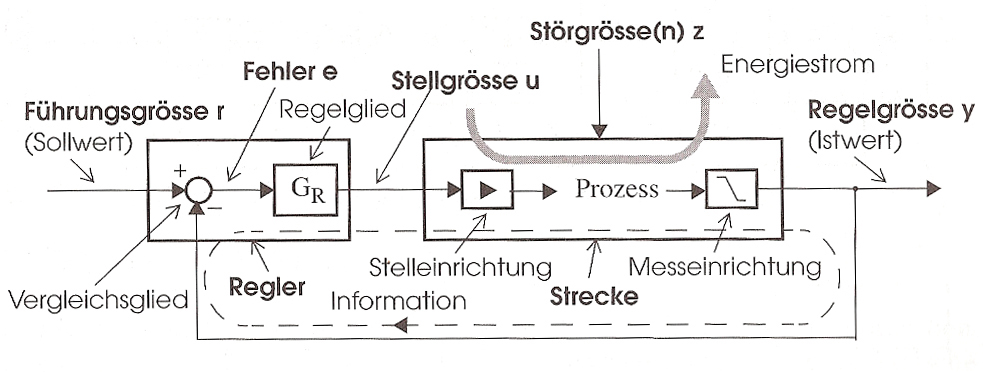
\includegraphics[height=4.5cm]{./bilder/Grundregelkreis_klein.jpg}


		
		\begin{sidewaystable}
		\subsection{Klassifizierung technischer Systeme}
		\begin{tabular}{|p{3cm}|p{2.5cm}|p{7cm}|p{11.5cm}|}
        	\hline
        	
        	einfach &
        	schwierig &
        	\textcolor{red}{\underline{für Regler}} &
        	Bedeutung des ersten Begriffs\\
        	\hline
        	
        	statisch &
        	\textcolor{red}{\underline{dynamisch}} &
        	&
        	Beschreiben nur den Gleichgewichtszustand (Vorgeschichte nicht
        	berücksichtigt)\\
        	\hline
        	
        	\textcolor{red}{\underline{linear}}	&
        	nichtlinear &
        	Ausnahmen: 2-, 3-Pt.Regler Simulation &
        	Assoziativ und Kommutativgesetz berücksichtigt \newline (x=X, 2x=2X;
        	y=Y, x+y=X+Y)\\
        	\hline
        	
        	\textcolor{red}{\underline{zeitinvariant}} &
        	zeitvariant &
        	&
        	unabhängig von zeitlicher Verschiebung \\
        	\hline
        	
        	\textcolor{red}{\underline{Zeitkontinuierlich}} &
        	zeitdiskret &
        	&
        	Signal hat zu jedem Zeitpunkt einen Wert\\
        	$\dot{y}=\frac{ku-y}{T}$ &
        	$y_{k+1}=a y_k + b u_k$	&
        	&
        	\\
        	\hline
        	
        	\textcolor{red}{\underline{wertkontinuierlich}}&
        	wertdiskret&
        	&
        	Signal kann alle Werte eines Intervalles annehmen\\
        	\hline
        	
        	\textcolor{red}{\underline{kausal}}	&
        	akausal	&
        	&
        	Gleiche Ursache führt zur gleichen Wirkung\\
        	\hline
        	
        	\textcolor{red}{\underline{konzentrierte}} &
        	verteilte &
        	zB.	Stromleitung: &
        	\\
        	\textcolor{red}{\underline{Parameter}} &
        	Parameter	&
        	ein R und ein C/ sehr viele RC-Glieder in Serie &
        	\\
        	\hline
        	
        	\textcolor{red}{\underline{deterministisch}}	&
        	stochastisch &
        	vorhersehbar/zufällig &
        	Das Zeitverhalten lässt sich aufgrund seiner Gleichungen
        	``reproduzieren"\\
        	\hline
        \end{tabular}
        \end{sidewaystable}	
\section{Regelungen}
\subsection{Glieder}

	\begin{tabular}{|l|l|l|l|l|l|}
    	\hline
    	\textbf{Benennung}	&\textbf{Funktion}	&\textbf{UTF}	& \textbf{Sprungantw.}	
    		&\textbf{Verlauf Sprungantw.}	&\textbf{Symbol}\\
    	\hline
    	\hline
    	\textbf{P-Glied} \formelbuch{35} & $y(t)=K u(t)$	& K & K
    	&\begin{minipage}{2.4cm}
         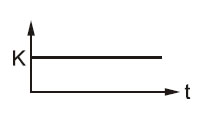
\includegraphics[width=2.4cm,trim=0 0 -5 -5]{./bilder/verlaufP.jpg}
         \end{minipage}
    	&\begin{minipage}{2.4cm}
         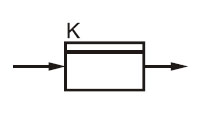
\includegraphics[width=2.4cm]{./bilder/p-Glied.jpg}
         \end{minipage}\\
    	\hline
    	\textbf{I-Glied} \formelbuch{28} &
    	\parbox{3cm}{$\dot{y}= K u(t)$\\
    				$y=K\int \limits_0^t u(t) dt$\\}
    				&$\dfrac{K}{s}$
    	&Kt
    	&\begin{minipage}{2.4cm}
         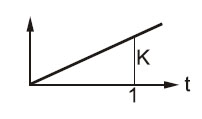
\includegraphics[width=2.4cm,trim=0 0 -5 -5]{./bilder/verlaufI.jpg}
         \end{minipage}
    	&\begin{minipage}{2.4cm}
         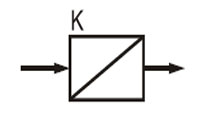
\includegraphics[width=2.4cm]{./bilder/I-Glied.jpg}
         \end{minipage}\\
    	\hline
    	
    	\textbf{Totzeit-Glied} \formelbuch{41}	
    	&$y(t)=u(t-T_t)$	&$e^{-T_t s}$	&$K \cdot u(t-T_t)$
    	&\begin{minipage}{2.4cm}
         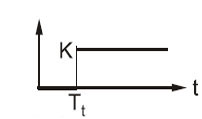
\includegraphics[width=2.4cm,trim=0 0 -5 -5]{./bilder/verlaufTt.jpg}\\
         \end{minipage}
    	&\begin{minipage}{2.4cm}
         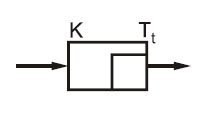
\includegraphics[width=2.4cm]{./bilder/Tt-Glied.jpg}
         \end{minipage}\\
		\hline
    	 \begin{minipage}{4cm}
			\vspace{0.2cm}
			\textbf{PT$_1$-Glied} \formelbuch{37}\\
			%    	   	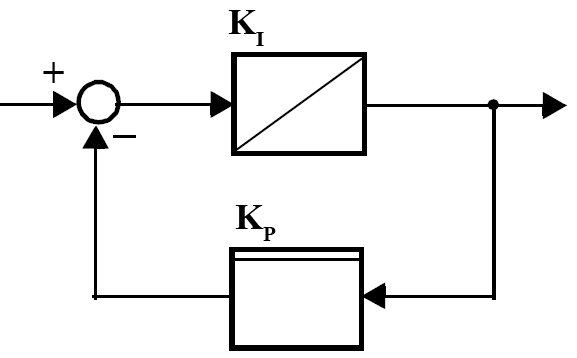
\includegraphics[width=4cm]{./bilder/PT1.png}   
         \end{minipage}
		 &\parbox{3cm}{$T\dot{y}+y=K u(t)$\\\\
		 $T = \dfrac{1}{K_i \cdot K_p}$\\
		 $K = \dfrac{1}{K_p}$}	 
		 &$\dfrac{K}{1+Ts}$
    	 &$K(1-e^{-\frac{t}{T}})$
    	 &\begin{minipage}{2.4cm}
         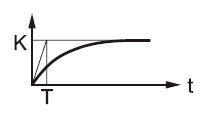
\includegraphics[width=2.3cm]{./bilder/verlaufPT1.jpg}
         \end{minipage}
    	&\begin{minipage}{2.4cm}
         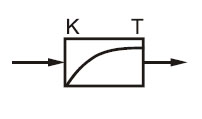
\includegraphics[width=2.3cm]{./bilder/Pt1-Glied.jpg}
         \end{minipage}\\
    	\hline
    	\multicolumn{6}{|l|}{
    		\parbox{18cm}{\textbf{PT$_1$-Glied mit Grundelementen} ($K$: Verstärkung; $T$: Zeitkonstante):\\
    				\begin{minipage}{10cm}
    				    \hspace*{4cm}
    				    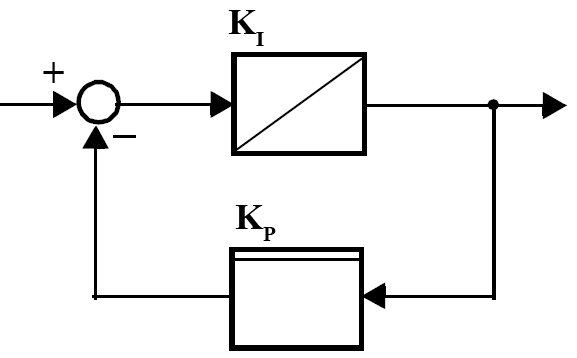
\includegraphics[width=4cm]{./bilder/PT1.png}
    				\end{minipage}
    				\begin{minipage}{7cm}
    					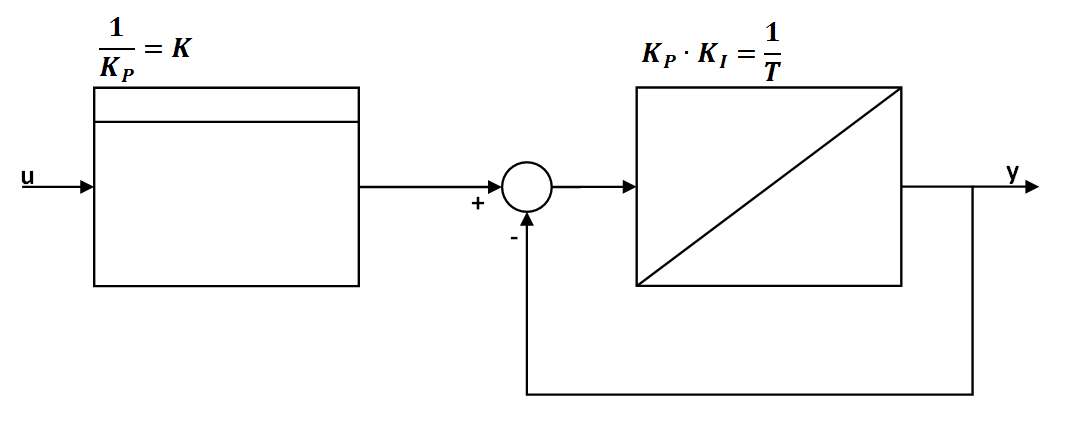
\includegraphics[width=6cm]{./bilder/PT1_2.png}
    				\end{minipage}
    		}
    	}\\
    	\hline

    \end{tabular}
		
    

    \begin{multicols}{3}
    \textbf{P-Glied (nicht inv. Op-Amp)} \\
    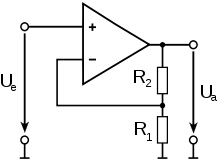
\includegraphics[height=2.5cm]{./bilder/OP-Amp.png} \\
    $K = 1 + \frac{R_2}{R_1}$ 
    \columnbreak

	\textbf{P-Glied (inv. Op-Amp)} \\ 
	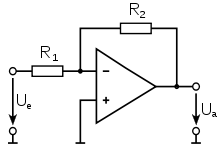
\includegraphics[height=2.5cm]{./bilder/OP-InvAmp.png} \\
	$K=-\frac{R_2}{R_1}$
    \columnbreak
        
    \textbf{I-Glied} \\ 
    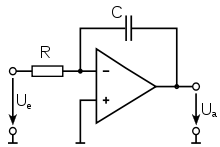
\includegraphics[height=2.5cm]{./bilder/OP-Integrator.png}\\
    $K = - \frac{1}{R \cdot C}$
    
    \end{multicols}
    
    
    \begin{minipage}{16cm}
    \subsection{Stationäre Signale}
	Für den stationären Fall gelten folgende Bedingungen:
	\begin{itemize}
    	\item \textbf{Integratoren} haben am \textbf{Eingang Null}.
    	\item \textbf{Integratoren} haben am \textbf{Ausgang} einen \textbf{beliebigen Wert}.
    	\item \textbf{Totzeitglieder} werden kurzgeschlossen.
    	\item \textbf{PT$_1$-Glieder} wirken als \textbf{P-Glieder} mit $K_P = K_{PT_1}$ behandelt.
    	\item (\textbf{Fehlersignale} werden jeweils als \textbf{Null} angenommen.) \textbf{Mit Vorsicht annehmen}
  	\end{itemize}
  	\end{minipage} \\


	\subsection{Zwei- und Dreipunktregler}

	\subsection{Stetigähnliche Regler}
		\subsubsection{Rückkopplung des Reglers}
		\begin{minipage}{9cm}
		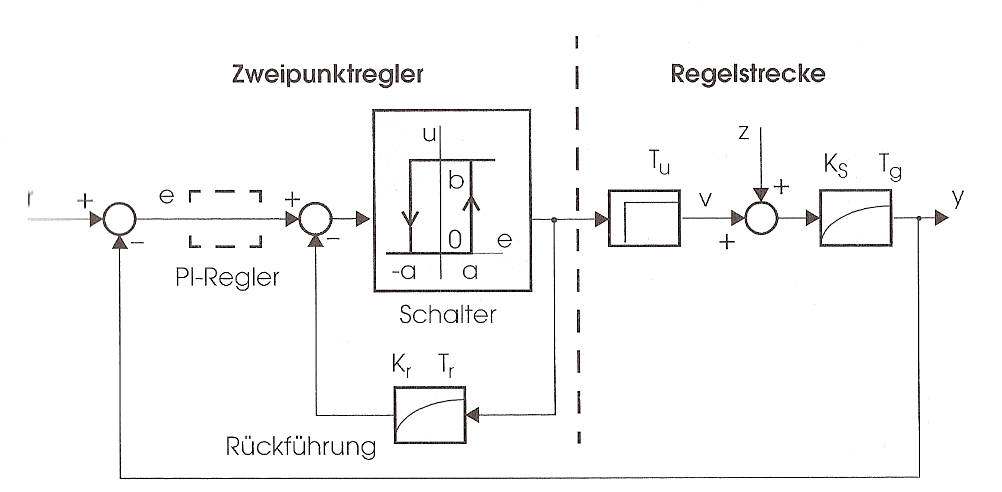
\includegraphics[width=8.5cm]{./bilder/ZweipunktreglerMitRueckfuehrung.jpg}
        \end{minipage}
		\begin{minipage}{7.5cm}
        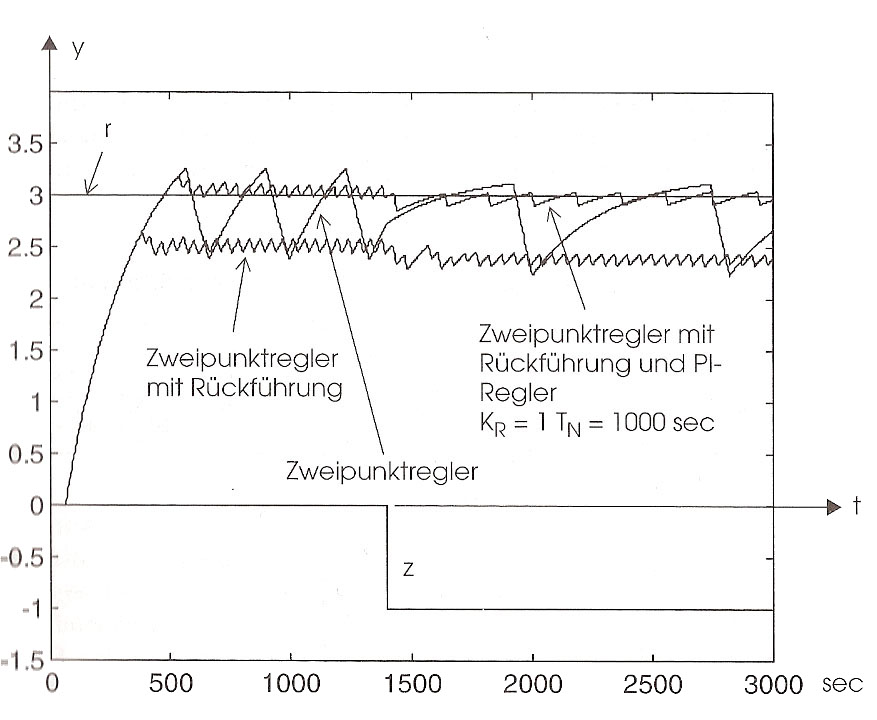
\includegraphics[width=7cm]{./bilder/ZweipunktreglerMitRueckfuehrung_dia.jpg}
        \end{minipage}\\
		Die Rückkopplung mit einem $PT_1$-Glied über dem Zweipunkteregler bewirkt
		einen bedeutend kleineren Rippel. Leider ist der Mittelwert noch unterhalb des
		Sollwertes. Mithilfe eines PI-Reglers vor dem Zweipunkteregler, kann der IST-Wert
		angehoben werden.
	
	\subsubsection{Dreipunktregler}
		\begin{minipage}{9cm}
		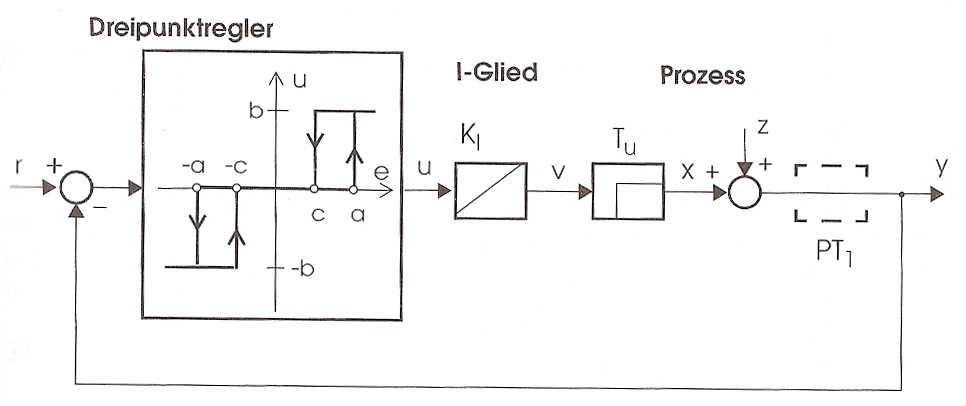
\includegraphics[width=9cm]{./bilder/Dreipunktregler.jpg}
        \end{minipage}
		\begin{minipage}{7.5cm}
        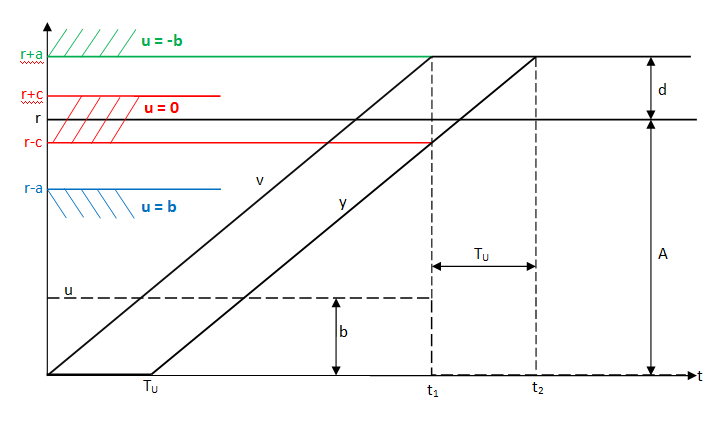
\includegraphics[width=7.5cm]{./bilder/Dreipunktregler_dia.png}
        \end{minipage}\\
		gewünscht: $d = 0 \rightarrow c = K_I \cdot T_u \cdot b$\\
		Falls mit PT$_1$-Glied $\rightarrow c = K_I \cdot K_s \cdot b (T_u + T_G)$
		
		
	\subsubsection{Zweipunktregler}
		\begin{minipage}{3cm}
 		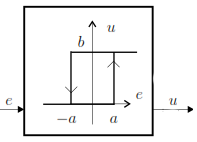
\includegraphics[height=3cm]{./bilder/Zweipunkteregler.png}
        \end{minipage}
		\begin{minipage}{15cm}
        Ein Zweipunktregler ist ein unstetig arbeitender Regler mit zwei
        Ausgangszuständen. Je nachdem, ob der Istwert über oder unter dem
        Sollwert liegt, wird der erste oder der zweite Ausgangszustand
        eingenommen. 
        \end{minipage}
        
	\textbf{Beispiele von Zweipunkte-Reglerschaltungen:}\\ \\
		\textbf{Zweipunktregler mit symmetrischer Kennlinie \formelbuch{52}} \\
		\begin{minipage}{9cm}
			\vspace{.5cm}        
	 		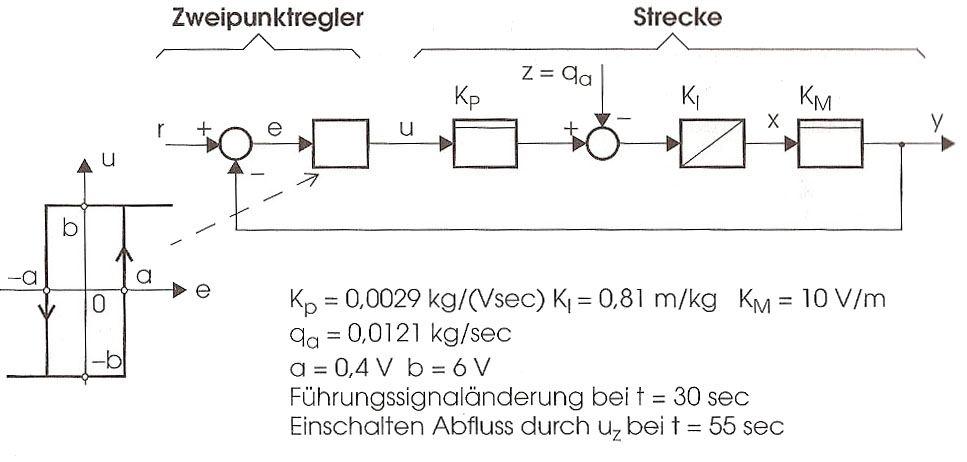
\includegraphics[width=9cm]{./bilder/Zweipunktregler-b+b2.jpg}\\
			Die Anstiegszeit beträgt nach dem Einschwingvorgang:\\
			$t_{ein}=\frac{2a}{(b K_p - q_a)K_i K_m}$ \\ \\
			Die Abfallszeit beträgt nach dem Einschwingvorgang:\\
			$t_{aus}=\frac{2a}{(b K_p + q_a)K_i K_m}$
        \end{minipage}
		\begin{minipage}{9cm}
			\vspace{.5cm}        
			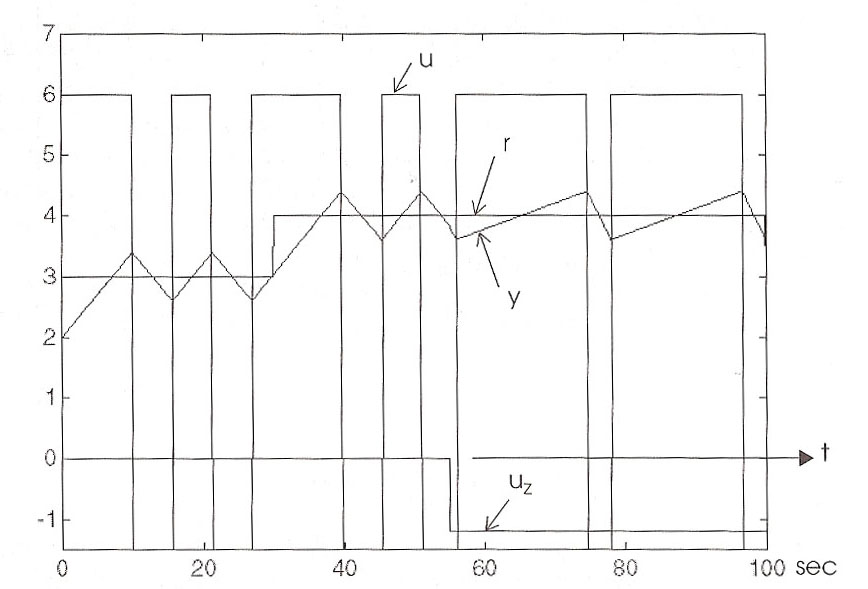
\includegraphics[width=9cm]{./bilder/Zweipunktregler-b+b_dia.jpg}
        \end{minipage}\\
         Einfüllen mit Abfluss: $y = y_0 + K_M \cdot K_I(K_p \cdot b - Q_a)(t-t_0); \qquad$ 
         Entleeren: $y=y_1 + K_M \cdot K_I(K_p(-b) - Q_a)(t-t_0)$
         

	\vspace{.5cm}
		\textbf{Zweipunktregler an ausgleichender Strecke \formelbuch{53}} \\
		\begin{minipage}{9cm}
 		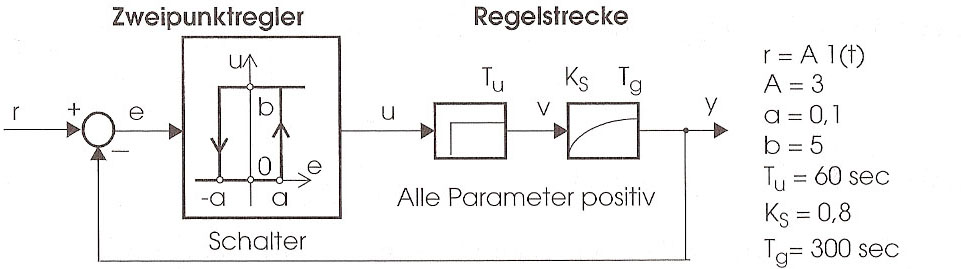
\includegraphics[width=9cm]{./bilder/ZweipunktreglerTotglied2.jpg}\\
			Die Anstiegszeit beträgt nach dem Einschwingvorgang:
			$t_{ein}$=$T_g\ln(\frac{e^{-\frac{T_u}{T_g}}(A-a)-b K_s}{A+a-b K_s})+T_u$\\ \\
			Die Abfallszeit beträgt nach dem Einschwingvorgang:
			$t_{aus}$=$T_g\ln(\frac{A+a-b
			K_s+\frac{b K_s}{e^{-\frac{T_u}{T_g}}}}{A-a})$\\
        \end{minipage}
		\begin{minipage}{9cm}
		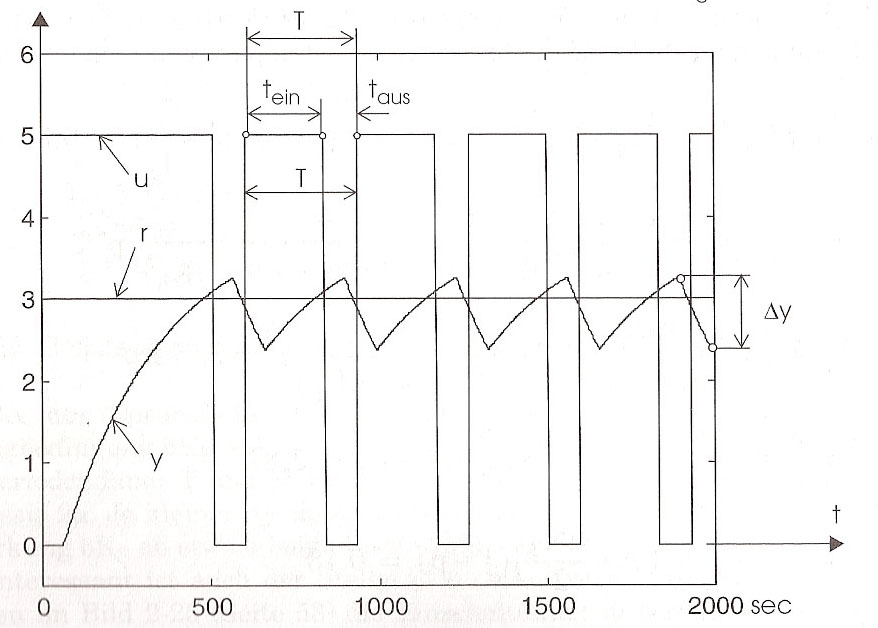
\includegraphics[width=9cm]{./bilder/ZweipunktreglerTotglied_dia.jpg}			
        \end{minipage}
    
 	$\Delta y = b\cdot K_s - e^{-\frac{T_u}{T_G}}(b\cdot K_s - 2a); \qquad$
	$y_m = \frac{y_{min}+y_{max}}{2}=e^{-\frac{T_u}{T_G}}\cdot A + \frac{b\cdot K_s}{2}(1-e^{-\frac{T_u}{T_G}}$


\section{Linearisierung \formelbuch{76}}
	\begin{minipage}[c]{10cm}
		\subsection{LTI-Systeme \formelbuch{83}}
			\renewcommand{\arraystretch}{1.5}
			\begin{tabular}{|l|l|}
				\hline
				\textbf{Linearität} & \textbf{Zeitinvarianz}\\
				\hline
				$\Phi(x1+x2)=\Phi(x1)+\Phi(x2)$ & $\Phi(x(t-t_0)=\Phi(x)\cdot x(t-t_0)$ \\
				$\Phi(c\cdot x)=c\cdot \Phi(x)$ & \\
				\hline    
			\end{tabular}
			\renewcommand{\arraystretch}{1}
		\end{minipage}
		\begin{minipage}[c]{6cm}
			\subsection{Linearitätstest \formelbuch{80}}
			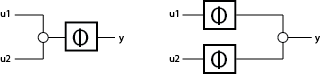
\includegraphics[width=6cm]{bilder/linearitaetstest}
		\end{minipage} \\
		
	\subsection{Linearität in den Parametern}
		Eine Funktion $f$ ist linear in den Parametern, wenn sie durch eine Linearkombination der Parameter geschrieben werden kann: \\
		$f(t) = \sum\limits_{j=1}^m a_j \cdot f_j(t)$ \\
		Beispiel: $y = \left[\begin{matrix} u & w \end{matrix} \right] \cdot \left[\begin{matrix} a_1 \\ a_2 \end{matrix}\right]$ ist linear in den Parametern $a$
	
	\subsection{Einfluss der Lage einer Nichtlinearität}
		\begin{enumerate}
			\item	nicht lineare Komponente dürfen \underline{nicht} vertauscht werden!\\
			\item vertauschen von linearen Blöcken erlaubt falls ...\\
								... Anfangsbedingung = 0\\
								... interne Signale keine Rolle spielen
		\end{enumerate}
	  	
	\subsection{Erwünschte Nichtlinearität \formelbuch{84}}
		In einem Prozess sind Linearitäten meist erwünscht, da sie meist mit
		Gleichungen zu lösen sind.
		Viele Efekte, wie zum Beispiel die Modulation oder so sind aber gerade erst
		durch Nichtlinearitäten möglich. Daher unterscheidet man:\\
	\begin{minipage}[c]{8cm}
		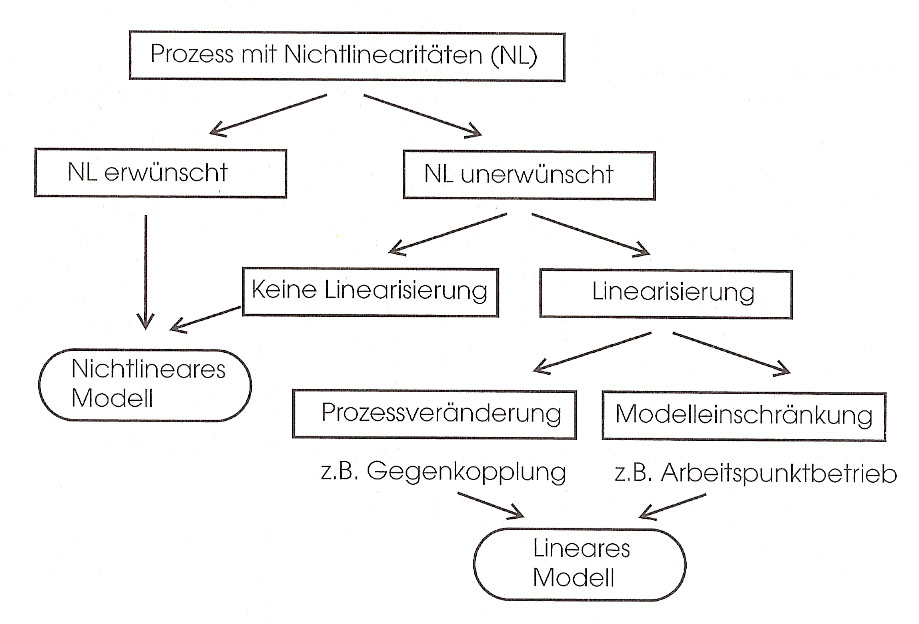
\includegraphics[width=8cm]{./bilder/Liste_Nichtlinearitaeten.jpg}
	\end{minipage}
	\begin{minipage}[c]{8cm}
		\textbf{Lineare Operationen} \\
		- Addition \\
		- Integration \\
		- Differentiation \\
		daraus folgt, dass folgende Glieder auch linear sind: \\
		- P-Glied \\
		- I-Glied \\
		- PT1-Glied
	\end{minipage}
	\subsection{Erfassen von nicht linearen Kurven}
	\subsubsection{Messung einer statischen Kennlinie \formelbuch{86}}
	\begin{minipage}{10cm}
		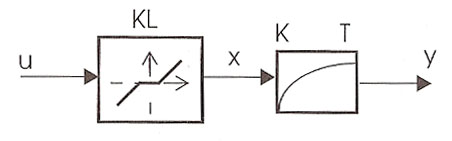
\includegraphics[width=7cm]{./bilder/NichtlinearMitPT1.jpg}   
    \end{minipage}
	\begin{minipage}{7cm}
    	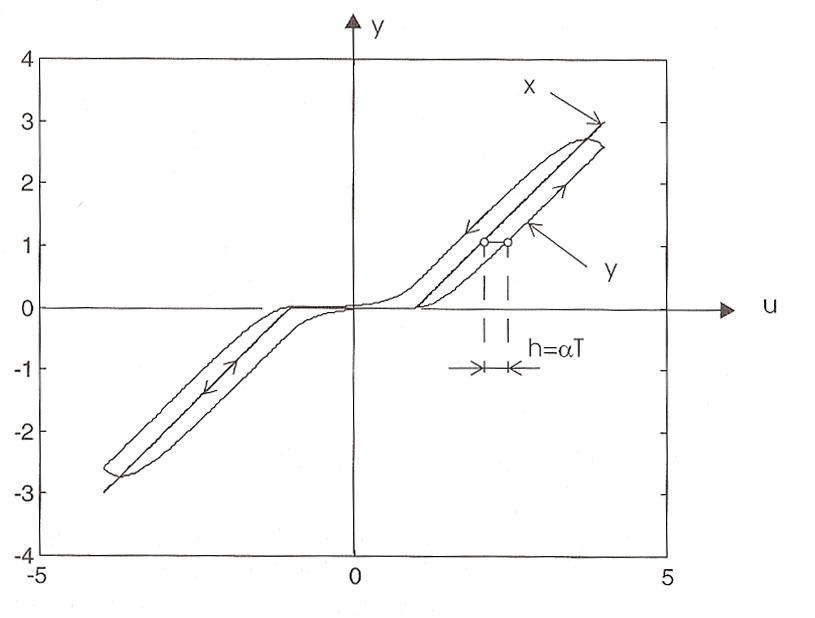
\includegraphics[width=5cm]{./bilder/NichtlinearMitPT1_dia.jpg}
    \end{minipage}\\
		Da das Signal x meist nicht zugänglich ist, muss man den ganzen Prozess
		ausmessen.\\
		Mit einem Dreieck kann man die Kennlinie auslesen. Sie wird jedoch von einer
		``unechten" Hysterese verzerrt, die eine Hysteresebreite von 2$\alpha$ T, wobei
		$\alpha$ die Rampensteilheit ist und T die Zeitkonstante des PT1-Gliedes.

	\subsubsection{Mathematische Erfassung einer Messkurve \formelbuch{89}}
	\begin{floatingfigure}[r]{12cm}
    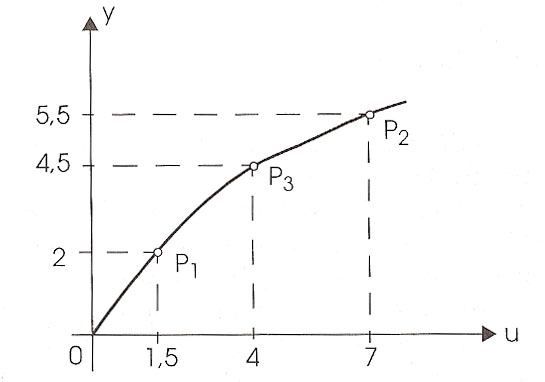
\includegraphics[width=10cm,height=3cm]{./bilder/KennlinieMitStuetzwerten.jpg}
	\end{floatingfigure}
   	
     	\begin{enumerate}
     	\item \textbf{Wahl einer geeigneten Funktion:}\\
     	Gesucht ist ein Graph, der eine ähnliche Form
		hat wie die Messkurve. Günstig sind Polynome, da sie mathematisch einfach zum
		beschreiben sind, aber auch Sinus- oder Arctan- Funktionen	\\ 
        \\
     	
        \item \textbf{Bestimmung der Parameter:}
          \begin{enumerate}
           \item Methode der ausgewählten Punkte:\\
          		\begin{enumerate}
                    \item Gleich viele Messpunkte wie frei zu wählende Parameter der
           			Approximationsfunktionen.
           			\item Einsetzen der Koordinaten der Messpunkte in die Gleichungen.
           		\end{enumerate}
           	\item Methode der kleinsten Fehlerquadrate:
           		\begin{enumerate}
                     \item Mindestens gleich viele Messpunkte wie Parameter der
           		Appxomationsfunktion, können jedoch mehr gewählt werden. z.B. \\
						Näherungsfunktion: $y = ax^2 + bx$ \\
						P1:		$2.0 = a\cdot 1.5^2+b\cdot 1.5$ \\
						P2: 	$5.5 = a\cdot 7^2+b\cdot 7$\\
						P3: 	$4.5 = a\cdot 4^2+b\cdot 4$         		
           		\item Fehler bilden zwischen Messpunkt und Funktionspunkt. z.B.\\
           		\begin{minipage}{10cm}
           				P1:  	$e_1=2-y=2-(a(1.5)+b(1.5)^2)$\\
           				P2:  	$e_2=5.5-y=5.5-(a(7)+b(7)^2)$\\
           				P3:  	$e_3=4.5-y=4.5-(a(4)+b(4)^2)$\\
           		\end{minipage}
				\begin{minipage}{6cm}
					\textbf{Matrixschreibweise:}\\
						$\left[\begin{matrix}
						2.0 \\5.5\\ 4.5
						\end{matrix}\right] =
						\left[\begin{matrix}
						1.5^2 & 1.5 \\ 7^2 & 7\\ 4^2 & 4
						\end{matrix}\right] \cdot
						\left[\begin{matrix}
						a \\ b
						\end{matrix}\right] \Rightarrow
						\vec{y} = M \cdot \vec{p}$
				\end{minipage}\\           		
           		\item Nach Gauss ist die beste Näherung, wenn die Summe der
           		Fehlerquadrate minimal wird. \\
           		\begin{minipage}{8cm}
           			$\Longrightarrow$ S =$ e_1^2+e_2^2+e_3^2=min$\\
           			$\frac{\delta S}{\delta a}=
           			2 e_1 \frac{\delta e_1}{\delta a}+
           			2 e_2 \frac{\delta e_2}{\delta a}+
           			2 e_3 \frac{\delta e_3}{\delta a}=0$\\
           			$\frac{\delta S}{\delta b}=
           			2 e_1 \frac{\delta e_1}{\delta b}+
           			2 e_2 \frac{\delta e_2}{\delta b}+
           			2 e_3 \frac{\delta e_3}{\delta b}=0$\\
           		\end{minipage}
				\begin{minipage}{9cm}
					\textbf{mit Matrizen:}\\
						$M$ nicht überbestimmt: $\vec{p} = M\backslash\vec{y} = M^{-1} \cdot \vec{y} \rightarrow$ \\
						$M$ überbestimmt: $\vec{p} = pinv(M)\cdot \vec{y} = (M^TM)^{-1}M^T \cdot \vec{y}$\\
				\end{minipage}           		
           		\item Nachteil dieser Methode ist, dass es meist einen grossen
           		Rechenaufwand ergibt. Sie ist jedoch genauer als die erste Methode.
           		Ausserdem geht die Approixmationsfunktion nicht durch die Messwerte.
           		\end{enumerate}
		\end{enumerate}
	\end{enumerate}
	
\newpage

	\subsection{Linearisierung}
		\subsubsection{Modelleinschränkung \formelbuch{92}}
			Praktisch alle physikalische Systeme unterliegen gewissen Aussteuergrenzen.
			In diesen können sie linear sein. Es muss darauf achten, dass  das System
			diese nicht überschreitet. \\
			z.B. Festwert-Regelung: Die Kennlinie wird nur beim Einschalten durchlaufen.
			Ab dann bewegt sich die Regelung nur in einem sehr kleinen Bereich um den
			Arbeitspunkt, wo die Kennlinie linearisiert werden kann. \\
			
		\subsubsection{Arbeitspunkt \formelbuch{93}}
			Wenn eine Kennlinie für einen bestimmten Aussteuerung einen nicht zu grosse
			Krümmung hat, kann man in der Näherung diese durch die Tangente ersetzen, und
			somit wieder linear rechnen. \\
			Trigonometrische Funktionen bei Arbeitspunkt $\alpha = 0$: $\qquad \sin \alpha \approx
			\alpha \qquad \tan \alpha \approx \alpha \qquad \cos \alpha \approx 1$ \\
			\textbf{Vorgehen} \\
			\begin{minipage}[c]{6cm}
				\includegraphics[width=6cm]{bilder/LinArbeitspunkt}
			\end{minipage}
			\begin{minipage}[c]{12cm}
				\begin{enumerate}
					\item DGL des Systems bestimmen
					\item Alle Signale darstellen als $u(t)=u_0+\Delta u,\,v(t)=v_0+\Delta v,\dots$
					\item Arbeitspunkte $u_0,v_0,\dots$ = stationärer Zustand bestimmen
					\item Signaländerungen $\Delta u, \Delta v, \dots$ linearisieren
							(Tangente an Kennline)
					\item DGL durch Signaländerungen darstellen.
					\item Blockschaltbild mit Signaländerungen darstellen (siehe links)
				\end{enumerate}
			\end{minipage}
			
		\subsubsection{Durch inverse Kennlinie \formelbuch{94}}
		\begin{minipage}{11cm}
			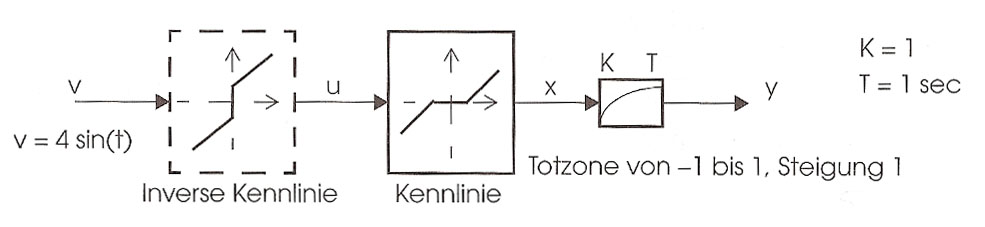
\includegraphics[width=10cm]{./bilder/Kennlinienkompensation.jpg}
        \end{minipage}
		\begin{minipage}{6cm}
        	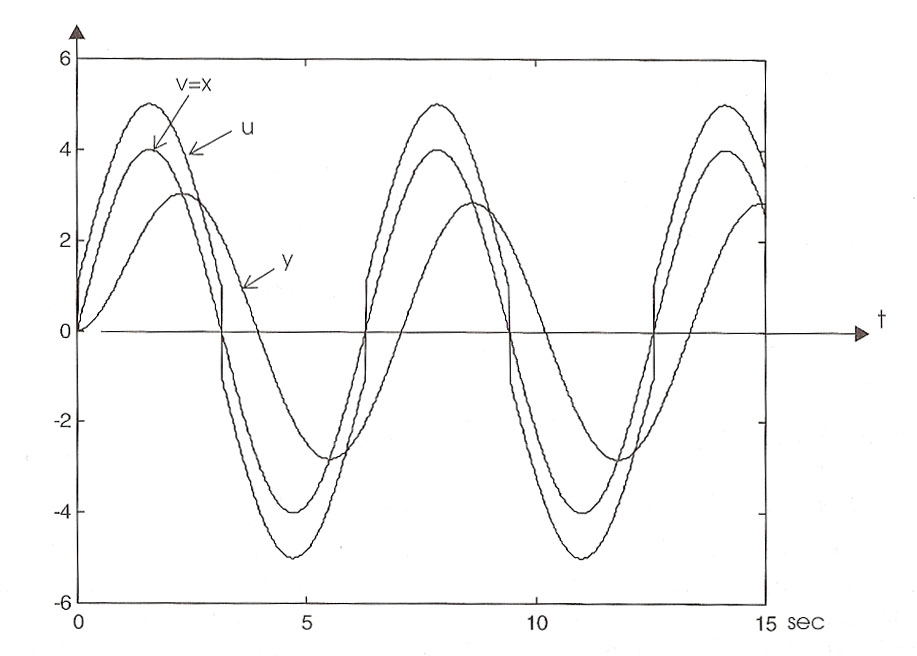
\includegraphics[width=6cm]{./bilder/Kennlinienkompensation_dia.jpg}
        \end{minipage}\\
			Durch das Vorschalten der Inversen Kennlinie kann man die Nichtlinearitäten
			beheben. Das System als ganzes reagiert nun linear, das Innere des System
			jedoch immer noch nicht, wie man an den Kennlinien gut erkennen kann.
			
		\subsubsection{Durch Gegenkopplung \formelbuch{96}}
				\begin{minipage}{11cm}
			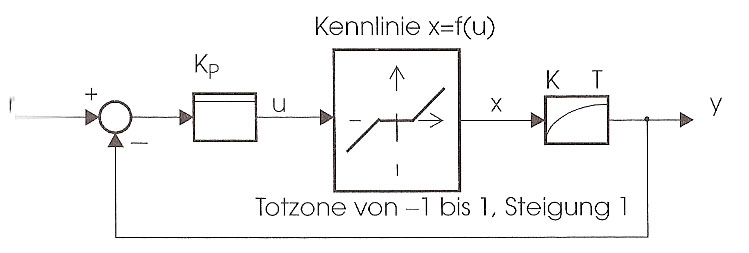
\includegraphics[width=10cm]{./bilder/Gegenkopplung.jpg}
        \end{minipage}
		\begin{minipage}{9cm}
        	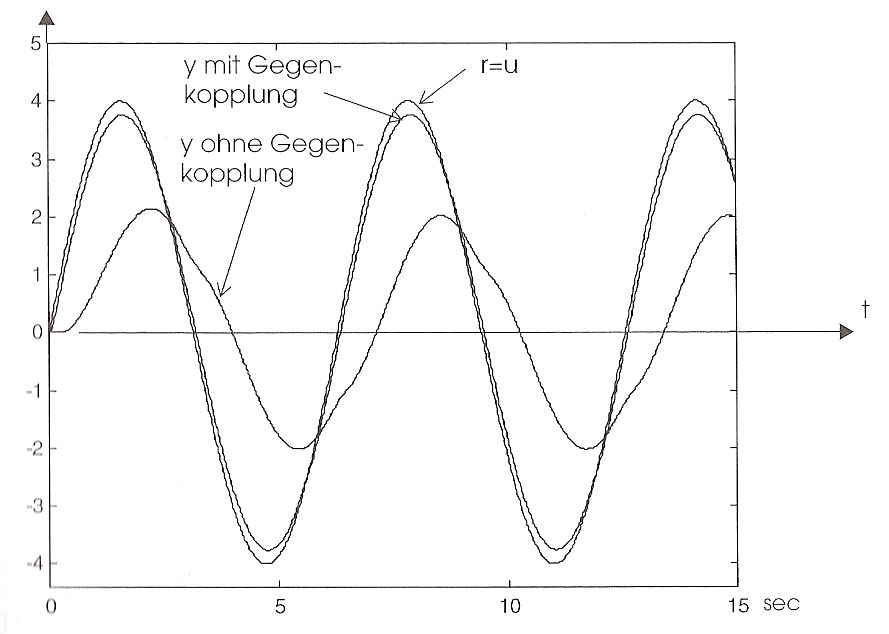
\includegraphics[width=6cm]{./bilder/Gegenkopplung_dia.jpg}
        \end{minipage}\\
			Da ein Prozess variierende Koefizienten besizten kann, kann die Kompensation
			nicht immer mit der inversen Kennlinie geschehen. Deshalb ist es oft
			günstiger die Nichtliniearitäten mit einer Gegenkopplung zu kompensieren.
			Diese ist umso wirksamer je grösser die Verstärkung $K_p$ ist.
			Es können jedoch Stabilitätsprobleme auftreten.


\section{Idiotenseite}
\input{idiotenseite/trigo/subsections/Winkelargumente}
\input{idiotenseite/diverses/subsections/kurven}
\input{idiotenseite/diverses/subsections/sivorsaetze}

\end{document}


